\documentclass[11pt,a4paper,oneside]{report}

% Size setup
\usepackage{anysize}
\marginsize{30mm}{30mm}{15mm}{15mm}

% Spacing setup
\setlength{\parindent}{2em} % Paragraph indenting
\setlength{\parskip}{0em} % Spacing between paragraphs
\frenchspacing

% Language setup
\usepackage[magyar]{babel} % Babel for Hungarian
\usepackage[T1]{fontenc} % Output character encoding
\usepackage[utf8]{inputenc} % Input character encoding
\selectlanguage{magyar}

% Notation setup
\usepackage{dsfont} % Number set fonts
\usepackage{physics} % Braket notation

% Image setup
\usepackage{graphicx} % Included graphics
\usepackage{subcaption} % Subfigures
\usepackage{float} % Fix image position

% Table setup
\usepackage[table]{xcolor} % Cell colors
% \usepackage{booktabs}
% https://jdhao.github.io/2019/08/27/latex_table_with_booktabs/

% Style setup
\usepackage[hidelinks]{hyperref} % Remove ugly rectangles around urls

% Bibliography setup
\usepackage[numbers]{natbib}
\bibliographystyle{acm}

\begin{document}

\pagenumbering{gobble}
\hypersetup{pageanchor=false}
%--------------------------------------------------------------------------------------
%	The title page
%--------------------------------------------------------------------------------------
\begin{titlepage}
\begin{center}

\includegraphics[width=60mm,keepaspectratio]{figures/bme_logo.pdf}\\
\vspace{0.3cm}
\textbf{\bme}\\
\textmd{\vik}\\
\textmd{\viktanszek}\\[5cm]

\vspace{0.4cm}
{\huge \bfseries \vikcim}\\[0.8cm]
\vspace{0.5cm}
\textsc{\Large \vikdoktipus}\\[4cm]

{
	\renewcommand{\arraystretch}{0.85}
	\begin{tabular}{cc}
	 \makebox[7cm]{\emph{\keszitette}} & \makebox[7cm]{\emph{\konzulens}} \\ \noalign{\smallskip}
	 \makebox[7cm]{\szerzo} & \makebox[7cm]{\vikkonzulensA} \\
	  & \makebox[7cm]{\vikkonzulensB} \\
	  & \makebox[7cm]{\vikkonzulensC} \\
	\end{tabular}
}

\vfill
{\large \today}
\end{center}
\end{titlepage}
\hypersetup{pageanchor=false}


\tableofcontents\vfill
\pagenumbering{arabic}

\chapter{Bevezetés}

A 20. századi fizika hatalmas változásokat hozott. A relativitáselmélet mellett
megjelent a kvantummechanika, mely teljesen megváltoztatta a világnézetünket.
Ugyanebben az időszakban kezdődött el a számítástechnika hajnala is.
Megjelentek az első számítógépek és elkezdték megírni az első programokat,
algoritmusokat.

Richard P. Feynman 1982-es cikkében fejtette ki, hogy a klasszikus
számítógépekkel sajnos csak exponenciális időben lehet kvantumjelenségeket
szimulálni, ez azonban túlságosan lassú a kísérletek elvégzéséhez. Ha viszont
lenne egy kvantumjelenségek alapján működő számítógépünk, akkor azzal
hatékonyan lehetne szimulációkat végezni, a fizikai kutatások elvégzéséhez. Így
született meg a kvantumszámítógép gondolata.

Benioff, Deutsch, majd Bernstein és Vazirani munkássága nyomán megszületett a
kvantum számítási modell, a kvantum Turing-gép a 80-as évek végére. Ettől
kezdve az a kérdés foglalkoztatja a kvantumalgoritmusok kutatóit, hogy vajon
vannak-e használható kvantumalgoritmusok, illetve vannak-e olyanok amik jobbak
mint a klasszikus párjaik.

Shor 1990-es kvantumon alapuló prímfaktorizációs algoritmusa már használható
algoritmus lett és az RSA alapú kódolás feltörésével fenyeget, ami komoly
veszélyt, illetve komoly előnyt is jelent azoknak akiknek van
kvantumszámítógépük. Erre már felfigyeltek a nagyhatalmak, multinacionális
cégek és szép lassan elkezdtek a kvantumszámítógépek kifejlesztésével
foglalkozni.

2019-ben a Google quantum supremacy bizonyítéka mutatott egy olyan
kvantumalgoritmust amely bár nem túl hasznos, de a mai legjobb
szuperszámítógépeket is megverte a Sicamore processzoruk teljesítménye.

Manapság egyre forróbb témává válik a kvantum és Magyarországon is egyre több
támogatás jut kvantummal kapcsolatos kutatásokra. A BME-n a Kvantuminformatikai
Nemzeti Labor tevékenykedik kvantumtitkosításon alapuló internet
kifejlesztésével és több tanszék, köztük a SZIT is bekapcsolódott a projektbe.

Ezen dolgozat a kvantumalgoritmusokon belül a kvantumbolyongásokkal
foglalkozik. A kvantumbolyongáson alapuló algoritmusokat azért érdemes kutatni,
mert több ismert kvantumalgoritmusnak az alapját képezik. A félév során
megismerkedtem a kvantuminformatika alapjaival, a gráfbolyongások klasszikus
illetve kvantumos változatával, valamint elkészítettem egy Pythonos
keretrendszert melyben könnyen lehet gráfbolyongásokkal kapcsolatos
kísérleteket, szimulációkat végezni.

A dokumentum hátralévő fejezeteiben bemutatom a kvantuminformatika alapjait,
ismertetem a klasszikus gráfbolyongást, továbbá a kvantumbolyongás egy
speciális esetét, bemutatom az elkészített Pythonos keretrendszert, majd
ismertetem a félév során kapott szimulációs eredményeket, végül a
továbbfejlesztési lehetőségekről beszélek.
\chapter{Klasszikus gráfbolyongások}

A klasszikus gráfbolyongások tulajdonképpen Markov-folyamatoknak felelnek meg.

A Markov-folyamat valószínűségi változóknak egy sorozata ($X_1, X_2, ..., X_n,
  ...$), melyek ugyanabból a diszkrét eloszlásból származnak és melyekre teljesül
a Markov-tulajdonság.

\paragraph{Markov-tulajdonság} A valószínűségi változók sorozatában az $(i+1).$
változó értéke csak az $i.$ változó értékétől függ, azaz $P(X_{i+1} = x_{i+1} |
  X_i = x_i, ..., X_1 = x_1) = P(X_{i+1} = x_{i+1} | X_i = x_i)$.

\paragraph{Homogén Markov-lánc} Olyan Markov-lánc melyben az átmeneti
valószínűség nem függ az időtől, azaz $P(X_{n+1} = i | X_n = j) = p_{i,j}$.

\paragraph{Átmeneti valószínűségi mátrix} A Markov-lánc átmeneti valószínűségi
mátrixa ezen $p_{i,j}$ elemekből áll.

\paragraph{Stacionárius eloszlás} Az $X_i$ változó eloszlása ha $i$ tart a
végtelenbe.

\paragraph{}

Egy ilyen Markov folymat megfeleltethető egy irányított súlyozott gráfnak,
a következő megkötésekkel:

\begin{itemize}
  \item A gráf csúcsai ultra thinmegfelelnek a valószínűségi változók (közös)
        értékkészletének az elemeinek.
  \item A $j.$ csúcsból au $i.$ csúcsba mutató él súlya $p_{i,j}$.
  \item Amennyiben $p_{i,j}=0$, úgy feltehető, hogy nem mutat él a $j.$
        csúcsból az $i.$ csúcsba.
\end{itemize}

\paragraph{}

Ezek alapján a Markov-lánc átmeneti valószínűségi mátrixa a fent definiált gráf
szomszédossági mátrixával egyezik. A gráfon klasszikus értelemben vett
bolyongást a következő módon végzünk:

\begin{itemize}
  \item Kiindulunk egy előre megadott csúcsból.
  \item A csúcsból kifele mutató élek közül a valószínűségeikkel súlyozva
        véletlenszerűen választunk egyet, ennek a végpontja lesz a következő csúcs.
  \item Meghatározott lépésig ismételjük az előző pontot.
\end{itemize}

\paragraph{}

Egy gráfon egyszerre több ilyen bolyongást is végezhetünk, párhuzamosan. A $k.$
lépésben hozzárendelhető a gráf csúcsaihoz, hogy aktuálisan hány bolyongó
helyezkedik el bennük. Megfelelően sok bolyongóval így közelíthető az
Markov-lánc $k.$ változójának az eloszlása.

Bolyongásokkal kapcsolatban többféle tulajdonságot szoktak mérni adott gráfon.

\paragraph{Keverési idő} A Markov lánc azon valószínűségi változójának az
indexe, melynek az eloszlása a stacionárius eloszlás $\epsilon$ sugarú
környezetében van.

\paragraph{Elérési idő} Az $i \leftarrow j$ csúcsok közötti elérési idő a
legkisebb szám, ahanyadik hatványra emelve az átmeneti valószínűségi mátrixot
az $i.$ sor $j.$ cellájában nemnulla érték szerepel.

\paragraph{}

A gyakorlatban sokféle közgazdaságtani, játékelméleti, statisztikus fizikából
ismert jelenséget modelleznek Markov-folyamatokkal. Ezek mellett gráfbolyongási
algoritmusokkal olyan problémák megoldását is fel lehet gyorsítani, a véletlen
bevezetésével, melyek alapból nem tartalmazzák azt. Például nagy méretű
gráfokban lehet ilyen módon részgráfokat keresni, de az internetes
keresőalgoritmusok (PageRank) is ezen az alapon működnek.

A kvantumbolyongásokat azért érdemes külön vizsgálni, mert esetükben a véletlen
választás teljesen másfajta módon működik, mint klasszikus esetben, erről a
következő fejezetben lesz szó.

\chapter{Kvantuminformatika}

Mielőtt a kvantumalgoritmusokkal elkezdhetünk foglalkozni, először meg kell
ismernünk a kvantuminformatika eszköztárát. Ez a fejezet Mika
Hirvensalo Quantum Computing című könyve \cite{Hirvensalo} alapján készült.

A klasszikus számítógépek esetében az információtárolás alapegysége a bit,
melynek értéke lehet 0 vagy 1. Kvantumszámítógépek esetében az alapegység a
kvantumbit, vagy röviden qubit. Kvantumbitek esetében a fizikai
tulajdonságaiknak köszönhetően az állapottér a komplex számokon értelmezett. A
legkisebb, kvantumszámításra használható állapottér 2 dimenziós.

\paragraph{Qubit} A 2 dimenziós Hilbert-tér ($H_2$) egy egységvektorát qubitnek
nevezzük. A tér bázisvektorai a $\ket{0}$ és az $\ket{1}$ ket vektorok.

Egy általános qubit tehát $c_0\ket{0} + c_1\ket{1}$ alakban írható fel, ahol
$c_0, c_1 \in{} \mathds{C}$ és $|c_0|^2 + |c_1|^2 = 1$.

\paragraph{Koordináta reprezentáció} A qubiteket koordinátákkal is lehet
reprezentálni, ekkor $\ket{0} = \begin{pmatrix} 1 \\ 0 \end{pmatrix}$, $\ket{1}
  = \begin{pmatrix} 0 \\ 1 \end{pmatrix}$ és $c_0\ket{0} + c_1\ket{1} =
  \begin{pmatrix} c_0 \\ c_1 \end{pmatrix}$.

\paragraph{Mérés} A kvantumbitek értéke ugyan bármely 1 hosszú vektor lehet a 2
dimenziós Hilbert-térben, azonban amikor ki szeretnénk olvasni az értéküket,
akkor a Hilbert-tér valamely bázisvektorát fogjuk kapni. A $c_0\ket{0} +
  c_1\ket{1}$ qubit esetében $|c_0|^2$ valószínűséggel kapjuk a $\ket{0}$ vektort
és $|c_1|^2$ valószínűséggel kapjuk a $\ket{1}$ vektort.

\paragraph{Tenzorszorzat} Az $r \times s$ méretű $A$ és $t \times u$ méretű $B$
mátrixok $rt \times su$ méretű $A \otimes B$ tenzorszorzata a következőképpen
definiált:

\begin{center}
  $A = \begin{pmatrix}
      a_{11} & a_{12} & \dots  & a_{1s} \\
      a_{21} & a_{22} & \dots  & a_{2s} \\
      \vdots & \vdots & \ddots & \vdots \\
      a_{r1} & a_{r2} & \ddots & a_{rs}
    \end{pmatrix}
  $
  és
  $B = \begin{pmatrix}
      b_{11} & b_{12} & \dots  & b_{1u} \\
      b_{21} & b_{22} & \dots  & b_{2u} \\
      \vdots & \vdots & \ddots & \vdots \\
      b_{t1} & b_{t2} & \ddots & b_{tu}
    \end{pmatrix}
  $ esetén
\end{center}

\begin{center}
  $A \otimes B = \begin{pmatrix}
      a_{11}B & a_{12}B & \dots  & a_{1s}B \\
      a_{21}B & a_{22}B & \dots  & a_{2s}B \\
      \vdots  & \vdots  & \ddots & \vdots  \\
      a_{r1}B & a_{r2}B & \ddots & a_{rs}B
    \end{pmatrix}
  $
\end{center}


\paragraph{Kvantumregiszter}

Az n qubites kvantumregiszter n darab qubit ($H_2$) tenzorszorzata.
$H_2^n = H_2 \otimes H_2 \otimes ... \otimes H_2$.

\section{Kvantumkapuk}

Az unitér mátrixok jelképezik a lehetséges fizikai operációkat a
kvantumbiteken. Egy ilyen unitér mátrix a Hadamard-mátrix, melyhez a
Hadamard-kapu tartozik.

\paragraph{Hadamard mátrix}

\begin{center}
  $H = \frac{1}{\sqrt{2}}\begin{pmatrix}
      1 & 1  \\
      1 & -1
    \end{pmatrix}$
\end{center}

\section{Hadamard-féle kvantumérme}

A Hadamard-féle kvantumérme egy olyan qubit, melynek a kiindulási állapota a $c
  = \ket{0}$ vagy $c = \ket{1}$ vektor és ha feldobjuk, akkor a
Hadamard-mátrixszal szorzódik.

Klasszikus érmék esetében ha feldobjuk 1-szer akkor $50\%$ eséllyel kapunk
fejet, $50\%$ eséllyel pedig írást. Kvantumérmék esetében 1-szer feldobás után
hasonló a helyzet. Például $\ket{0}$-ból kiindulva $H\ket{0} =
  \frac{1}{\sqrt{2}}\ket{0} + \frac{1}{\sqrt{2}}\ket{1}$, tehát
$(\frac{1}{\sqrt{2}})^2 = \frac{1}{2}$ valószínűséggel kapunk majd $\ket{0}$,
illetve $\ket{1}$ vektort ha megmérjük a kvantumérmét a feldobás után.

Klasszikus érmékre a második feldobás után a helyzet hasonló: $50\%$ eséllyel
kapunk fejet, $50\%$ eséllyel pedig írást. Kvantumérmék esetében azonban
érdekes jelenség figyelhető meg: $H^2\ket{0} = H(\frac{1}{\sqrt{2}}\ket{0} +
  \frac{1}{\sqrt{2}}\ket{1}) = \ket{0}$, hiszen a Hadamard-mátrix négyzete az
identitás mátrix. Tehát a 2. feldobás után $100\%$ valószínűséggel a kiindulási
értéket fogjuk visszakapni.

Klasszikus gráfbolyongások vizsgálatánál ha 2-reguláris gráfról van szó, akkor
a szomszéd véletlenszerű kiválasztása megfeleltethető egy klasszikus
érmefeldobás eredményének. Ebből a megfigyelésből kiindulva definiálhatjuk a
kvantum gráfbolyongást 2-reguláris gráfok esetén a kvantumérme
felhasználásával. A fenti eredményekből látszik, hogy nagyon más viselkedésre
lehet számítani, ezért érdemes ezzel a továbbiakban részletesen foglalkozni.

\chapter{Kvantumséta}

A kvantumbolyongásokat 2-reguláris gráfok esetén tehát a Hadamard-mátrix
segítségével definiáljuk. A következőkben az egyenesen, mint 2-reguláris gráfon
vett bolyongást fogjuk részletesen megvizsgálni. Ez a fejezet Susan Stepney
Quantum walking című írása \cite{Stepney} alapján készült.

Tegyük fel, hogy a bolyongás az egyenesen az origóból indul és a $k.$ lépés
után megáll. Ekkor a pozíció tárolására elegendő egy $(2k+1)$ méretű
állapotvektor, hiszen legfeljebb $k$ messzire juthatunk mindkét irányban a
kezdőponttól. Jelöljük ezt $\ket{P}$-vel és legyen $\ket{P}=(p_{-k}, ..., p_0,
  ..., p_{k})$, ahol $p_i\in\mathds{C}$ $\forall i$-re és $\sum\limits_{i=-k}^{k}
  |p_i|^2 = 1$. Azt mondjuk, hogy annak a valószínűsége, hogy a bolyongó éppen az
$i.$ koordinátán van $|p_i|^2$. Ezáltal egy teljes valószínűségi eloszlást
kaptunk a bolyongó pozíciója szerint.

Mivel kezdetben a bolyongó az origóban van, ezért a hozzá tartozó állapotvektor
$\ket{P_0} = (0, ..., 0, 1, 0, ..., 0)$, vagyis $p_0=1$, a többi $0$. A kvantumérme
kiindulási állapota pedig legyen $\ket{C_0} = \begin{pmatrix} \frac{1}{\sqrt{2}} \\
    \frac{i}{\sqrt{2}}\end{pmatrix}$. Ekkor a teljes rendszer állapotát e kettő
tenzorszorzata fogja megadni:

\begin{center}
  $\ket{\Psi_0} = \ket{P_0} \otimes \ket{C_0}
    = \frac{1}{\sqrt{2}} \begin{pmatrix}
      p_{-k}         \\
      i\cdot{}p_{-k} \\
      \vdots         \\
      p_{0}          \\
      i\cdot{}p_{0}  \\
      \vdots         \\
      p_{k}          \\
      i\cdot{}p_{k}
    \end{pmatrix}
  $
\end{center}

A lépés ezek után két fázisból áll. Az első fázisban az érmével dobunk. Ahhoz, hogy
a $\ket{\Psi}$ vektorban az érme állapotát frissítsük, azt az $I_{2k+1} \otimes H$
mátrixszal kell beszorozni. Ez egy olyan $(4k+2) \times (4k+2)$ -es mátrix, mely
$2 \times 2$-es almátrixokból áll és az átlójában Hadamard-mátrixok vannak:

\begin{center}
  \[ \hat{C} =
    \left(
    \begin{array}{cc|cc|cc|cc|cc|cc|cc}
        \frac{1}{\sqrt{2}} & \frac{1}{\sqrt{2}}  & 0      & 0      & \dots              & \dots               & \dots              & \dots               & \dots              & \dots               & \dots  & \dots  & 0                  & 0                   \\
        \frac{1}{\sqrt{2}} & -\frac{1}{\sqrt{2}} & 0      & 0      & \dots              & \dots               & \dots              & \dots               & \dots              & \dots               & \dots  & \dots  & 0                  & 0                   \\ \hline
        0                  & 0                   & \ddots &        & \ddots             &                     & \ddots             &                     & \ddots             &                     & \ddots &        & \vdots             & \vdots              \\
        0                  & 0                   &        & \ddots &                    & \ddots              &                    & \ddots              &                    & \ddots              &        & \ddots & \vdots             & \vdots              \\ \hline
        \vdots             & \vdots              & \ddots &        & \frac{1}{\sqrt{2}} & \frac{1}{\sqrt{2}}  & 0                  & 0                   & \ddots             &                     & \ddots &        & \vdots             & \vdots              \\
        \vdots             & \vdots              &        & \ddots & \frac{1}{\sqrt{2}} & -\frac{1}{\sqrt{2}} & 0                  & 0                   &                    & \ddots              &        & \ddots & \vdots             & \vdots              \\ \hline
        \vdots             & \vdots              & \ddots &        & 0                  & 0                   & \frac{1}{\sqrt{2}} & \frac{1}{\sqrt{2}}  & 0                  & 0                   & \ddots &        & \vdots             & \vdots              \\
        \vdots             & \vdots              &        & \ddots & 0                  & 0                   & \frac{1}{\sqrt{2}} & -\frac{1}{\sqrt{2}} & 0                  & 0                   &        & \ddots & \vdots             & \vdots              \\ \hline
        \vdots             & \vdots              & \ddots &        & \ddots             &                     & 0                  & 0                   & \frac{1}{\sqrt{2}} & \frac{1}{\sqrt{2}}  & \ddots &        & \vdots             & \vdots              \\
        \vdots             & \vdots              &        & \ddots &                    & \ddots              & 0                  & 0                   & \frac{1}{\sqrt{2}} & -\frac{1}{\sqrt{2}} &        & \ddots & \vdots             & \vdots              \\ \hline
        \vdots             & \vdots              & \ddots &        & \ddots             &                     & \ddots             &                     & \ddots             &                     & \ddots &        & 0                  & 0                   \\
        \vdots             & \vdots              &        & \ddots &                    & \ddots              &                    & \ddots              &                    & \ddots              &        & \ddots & 0                  & 0                   \\ \hline
        0                  & 0                   & \dots  & \dots  & \dots              & \dots               & \dots              & \dots               & \dots              & \dots               & 0      & 0      & \frac{1}{\sqrt{2}} & \frac{1}{\sqrt{2}}  \\
        0                  & 0                   & \dots  & \dots  & \dots              & \dots               & \dots              & \dots               & \dots              & \dots               & 0      & 0      & \frac{1}{\sqrt{2}} & -\frac{1}{\sqrt{2}} \\
      \end{array}
    \right)
  \]
\end{center}

A második fázisban a gráfon lépünk a következő csúcsba. Ahhoz, hogy balra lépjünk
a pozíció állapotvektorát egy olyan $S_{-}$ mátrixszal kell megszorozni, ami
az átló feletti 1-eseket tartalmaz:

\begin{center}
  \[ S_{-} =
    \left(
    \begin{array}{ccccc}
        0      & 1      & 0      & \cdots & 0      \\
               & \ddots & \ddots & \ddots & \vdots \\
        \vdots &        & \ddots & \ddots & 0      \\
               &        &        & \ddots & 1      \\
        0      &        & \cdots &        & 0
      \end{array}
    \right)
  \]
\end{center}

Ahhoz pedig, hogy jobbra lépjünk, egy olyan $S_{+}$ mátrixszal kell szorozni,
ami az átló alatti 1-eseket tartalmaz:

\begin{center}
  \[ S_{+} =
    \left(
    \begin{array}{ccccc}

        0      &        & \cdots &        & 0      \\
        1      & \ddots &        &        &        \\
        0      & \ddots & \ddots &        & \vdots \\
        \vdots & \ddots & \ddots & \ddots &        \\
        0      & \cdots & 0      & 1      & 0
      \end{array}
    \right)
  \]
\end{center}

Az érme $\ket{0}$ értékére lépünk balra, az $\ket{1}$ értékére pedig jobbra.
Tehát

\begin{center}
  \[ \hat{S} = S_{-}\ket{0}\bra{0} + S_{+}\ket{1}\bra{1}
  \]
\end{center}

Ami kifejtve,

\begin{center}
  \[ \hat{S} =
    \left(
    \begin{array}{cc|cc|cc|cc|cc|cc|cc}
        0                    & 0                    & \cellcolor{green!10} 1 & \cellcolor{green!10} 0 & 0                    & 0                    & \dots                  & \dots                  & \dots                  & \dots                  & \dots                & \dots                & 0                      & 0                      \\
        0                    & 0                    & \cellcolor{green!10} 0 & \cellcolor{green!10} 0 & 0                    & 0                    & \dots                  & \dots                  & \dots                  & \dots                  & \dots                & \dots                & 0                      & 0                      \\ \hline
        \cellcolor{red!10} 0 & \cellcolor{red!10} 0 & \ddots                 &                        & \ddots               &                      & \ddots                 &                        & \ddots                 &                        & \ddots               &                      & \vdots                 & \vdots                 \\
        \cellcolor{red!10} 0 & \cellcolor{red!10} 1 &                        & \ddots                 &                      & \ddots               &                        & \ddots                 &                        & \ddots                 &                      & \ddots               & \vdots                 & \vdots                 \\ \hline
        0                    & 0                    & \ddots                 &                        & 0                    & 0                    & \cellcolor{green!10} 1 & \cellcolor{green!10} 0 & \ddots                 &                        & \ddots               &                      & \vdots                 & \vdots                 \\
        0                    & 0                    &                        & \ddots                 & 0                    & 0                    & \cellcolor{green!10} 0 & \cellcolor{green!10} 0 &                        & \ddots                 &                      & \ddots               & \vdots                 & \vdots                 \\ \hline
        \vdots               & \vdots               & \ddots                 &                        & \cellcolor{red!10} 0 & \cellcolor{red!10} 0 & 0                      & 0                      & \cellcolor{green!10} 1 & \cellcolor{green!10} 0 & \ddots               &                      & \vdots                 & \vdots                 \\
        \vdots               & \vdots               &                        & \ddots                 & \cellcolor{red!10} 0 & \cellcolor{red!10} 1 & 0                      & 0                      & \cellcolor{green!10} 0 & \cellcolor{green!10} 0 &                      & \ddots               & \vdots                 & \vdots                 \\ \hline
        \vdots               & \vdots               & \ddots                 &                        & \ddots               &                      & \cellcolor{red!10} 0   & \cellcolor{red!10} 0   & 0                      & 0                      & \ddots               &                      & 0                      & 0                      \\
        \vdots               & \vdots               &                        & \ddots                 &                      & \ddots               & \cellcolor{red!10} 0   & \cellcolor{red!10} 1   & 0                      & 0                      &                      & \ddots               & 0                      & 0                      \\ \hline
        \vdots               & \vdots               & \ddots                 &                        & \ddots               &                      & \ddots                 &                        & \ddots                 &                        & \ddots               &                      & \cellcolor{green!10} 1 & \cellcolor{green!10} 0 \\
        \vdots               & \vdots               &                        & \ddots                 &                      & \ddots               &                        & \ddots                 &                        & \ddots                 &                      & \ddots               & \cellcolor{green!10} 0 & \cellcolor{green!10} 0 \\ \hline
        0                    & 0                    & \dots                  & \dots                  & \dots                & \dots                & \dots                  & \dots                  & 0                      & 0                      & \cellcolor{red!10} 0 & \cellcolor{red!10} 0 & 0                      & 0                      \\
        0                    & 0                    & \dots                  & \dots                  & \dots                & \dots                & \dots                  & \dots                  & 0                      & 0                      & \cellcolor{red!10} 0 & \cellcolor{red!10} 1 & 0                      & 0                      \\
      \end{array}
    \right)
  \]
\end{center}

A két fázist összevonva egy lépéshez a következő mátrix tartozik:

\begin{center}
  \[ \hat{U} = \hat{S} \cdot \hat{C} =
    (S_{-}\ket{0}\bra{0} + S_{+}\ket{1}\bra{1})\cdot\hat{C}
  \]
\end{center}

Ami kifejtve,

\begin{center}
  \[ \hat{U} =
    \left(
    \begin{array}{cc|cc|cc|cc|cc|cc|cc}
        0                    & 0                                      & \cellcolor{green!10} \frac{1}{\sqrt{2}} & \cellcolor{green!10} 0 & 0                    & 0                                      & \dots                                   & \dots                                  & \dots                                   & \dots                  & \dots                & \dots                                  & 0                                       & 0                      \\
        0                    & 0                                      & \cellcolor{green!10} \frac{1}{\sqrt{2}} & \cellcolor{green!10} 0 & 0                    & 0                                      & \dots                                   & \dots                                  & \dots                                   & \dots                  & \dots                & \dots                                  & 0                                       & 0                      \\ \hline
        \cellcolor{red!10} 0 & \cellcolor{red!10} \frac{1}{\sqrt{2}}  & \ddots                                  &                        & \ddots               &                                        & \ddots                                  &                                        & \ddots                                  &                        & \ddots               &                                        & \vdots                                  & \vdots                 \\
        \cellcolor{red!10} 0 & \cellcolor{red!10} -\frac{1}{\sqrt{2}} &                                         & \ddots                 &                      & \ddots                                 &                                         & \ddots                                 &                                         & \ddots                 &                      & \ddots                                 & \vdots                                  & \vdots                 \\ \hline
        0                    & 0                                      & \ddots                                  &                        & 0                    & 0                                      & \cellcolor{green!10} \frac{1}{\sqrt{2}} & \cellcolor{green!10} 0                 & \ddots                                  &                        & \ddots               &                                        & \vdots                                  & \vdots                 \\
        0                    & 0                                      &                                         & \ddots                 & 0                    & 0                                      & \cellcolor{green!10} \frac{1}{\sqrt{2}} & \cellcolor{green!10} 0                 &                                         & \ddots                 &                      & \ddots                                 & \vdots                                  & \vdots                 \\ \hline
        \vdots               & \vdots                                 & \ddots                                  &                        & \cellcolor{red!10} 0 & \cellcolor{red!10} \frac{1}{\sqrt{2}}  & 0                                       & 0                                      & \cellcolor{green!10} \frac{1}{\sqrt{2}} & \cellcolor{green!10} 0 & \ddots               &                                        & \vdots                                  & \vdots                 \\
        \vdots               & \vdots                                 &                                         & \ddots                 & \cellcolor{red!10} 0 & \cellcolor{red!10} -\frac{1}{\sqrt{2}} & 0                                       & 0                                      & \cellcolor{green!10} \frac{1}{\sqrt{2}} & \cellcolor{green!10} 0 &                      & \ddots                                 & \vdots                                  & \vdots                 \\ \hline
        \vdots               & \vdots                                 & \ddots                                  &                        & \ddots               &                                        & \cellcolor{red!10} 0                    & \cellcolor{red!10} \frac{1}{\sqrt{2}}  & 0                                       & 0                      & \ddots               &                                        & 0                                       & 0                      \\
        \vdots               & \vdots                                 &                                         & \ddots                 &                      & \ddots                                 & \cellcolor{red!10} 0                    & \cellcolor{red!10} -\frac{1}{\sqrt{2}} & 0                                       & 0                      &                      & \ddots                                 & 0                                       & 0                      \\ \hline
        \vdots               & \vdots                                 & \ddots                                  &                        & \ddots               &                                        & \ddots                                  &                                        & \ddots                                  &                        & \ddots               &                                        & \cellcolor{green!10} \frac{1}{\sqrt{2}} & \cellcolor{green!10} 0 \\
        \vdots               & \vdots                                 &                                         & \ddots                 &                      & \ddots                                 &                                         & \ddots                                 &                                         & \ddots                 &                      & \ddots                                 & \cellcolor{green!10} \frac{1}{\sqrt{2}} & \cellcolor{green!10} 0 \\ \hline
        0                    & 0                                      & \dots                                   & \dots                  & \dots                & \dots                                  & \dots                                   & \dots                                  & 0                                       & 0                      & \cellcolor{red!10} 0 & \cellcolor{red!10} \frac{1}{\sqrt{2}}  & 0                                       & 0                      \\
        0                    & 0                                      & \dots                                   & \dots                  & \dots                & \dots                                  & \dots                                   & \dots                                  & 0                                       & 0                      & \cellcolor{red!10} 0 & \cellcolor{red!10} -\frac{1}{\sqrt{2}} & 0                                       & 0                      \\
      \end{array}
    \right)
  \]
\end{center}

Az $i.$ lépés után tehát az aktuális $\Psi$ állapotvektor: $\ket{\Psi_i} =
  {\hat{U}}^i\cdot{}\ket{\Psi_0}$.

\paragraph{Mérés}

Annak a mérése, hogy a $i.$ koordinátán mekkora valószínűséggel van a bolyongó
a $j.$ lépésben.

Legyen $e_k$ egy $(2k+1)$ méretű csupa-0 vektor, kivéve az $i.$ koordinátát,
ahol 1 az értéke. Ekkor az állapotvektorból az i. koordinátához tartozó blokkot
az $\ket{e_k}\bra{e_k} \otimes \begin{pmatrix} 1 & 0 \\ 0 & 1 \end{pmatrix}$
mátrixszal történő beszorzással lehet kivágni:

\begin{center} \[ \ket{\phi_{i,j}} =
    (\ket{e_k}\bra{e_k} \otimes
    \begin{pmatrix} 1 & 0 \\ 0 & 1 \end{pmatrix})
    \cdot{} \ket{\Psi_j} \]
\end{center}

A blokkhoz tartozó valószínűség értéke az önmagával vett
(komplex) skalárszorzatának az eredménye lesz, azaz $\braket{\phi_{i,j}}$, ami valós.

Az ebben a fejezetben bemutatott algoritmust implementáltam a félév során. A 6.
fejezetben részletesen ismertetem az ezzel kapcsolatos szimulációs
eredményeket.
\chapter{Architektúra}

Ebben a fejezetben bemutatom az elkészült keretrendszert.

Programozási nyelvnek a Python 3-mat választottam. Ennek oka az, hogy nagyon
sok data science-el kapcsolatos modulja van, mely nagyban megkönnyíti a
különböző matematikai, algoritmuselméleti problémák feltárását, könnyen
iterálhatunk a különböző prototípusokon. Emellett a szintaxisa rövid, tömör,
lényegretörő programkódok megírását teszi lehetővé.

A forráskód három nagy részre bomlik:
\begin{itemize}
  \item Gráfmodellek
  \item Szimulátorok
  \item Futtatás, konfiguráció, eredmények ábragenerátora
\end{itemize}

\section{Gráfmodellek}

A félév során sokféle gráfon futtattam szimulációs kísérleteket, melyek során
több problémába ütköztem. Kezdetben úgy oldottam meg a szimulációkat, hogy a
cél gráfok szomszédossági mátrixait generáltam le, egyben a memóriában tartva
azokat és a lépések során a megfelelő csúcshoz tartozó sorokat lekérdezve.

Ezzel a módszerrel több probléma is jelentkezett. Az első gondot az okozta,
hogy a szomszédossági mátrix mérete a csúcsszám négyzetével arányos, ezért pár
ezer csúcsú gráfot már nem tudtam a memóriában tartva szimulálni. A második
probléma pedig az volt, hogy a szomszédossági mátrixos ábrázolás nagyon távol
esett az emberi szempontból természetes ábrázolástól. A kvantumbolyongásos
szimulációkat tipikusan nem véletlenszerű gráfokon szokták kipróbálni, hanem
jól ismert struktúrával rendelkező gráfokon. Ilyen gráfok például a súlyzó vagy
a ragasztott bináris fa gráfok.

A súlyzó gráf két egyforma méretű kört tartalmaz, mindkét körből kiválasztva
k-k darab csúcsot, melyek teljes páros gráfot alkotnak (a súlyzó középső
rúdját). A kör gráfokban pedig nem csak az egymás melletti csúcsok között fut
él, hanem futhat él minden i. csúcs között is. A ragasztott bináris fa gráf
pedig olyan, hogy két teljes bináris gráf leveleit szembefordítjuk és a két
oldali levelek közé egy teljes páros gráfot készítünk.

A fenti leírásból látható, hogy az ember számára természetes leírás a gráfokat
ismert részgráfok kompozitjaként adja meg. A félév során olyan architektúrát
alakítottam ki a szimulációkhoz, mely ezt a szemléletet támogatja. A
szomszédossági mátrixos tárolási mód helyett pedig a szomszédossági orákulum
megközelítést használva nagyban csökkent a memóriaigénye az alkalmazásnak.
Ennek a megközelítésnek a lényege, hogy az ismert struktúrájú gráfokra nem
tárolok a memóriában szomszédossági információt, helyette biztosítok egy
függvényt, amely a bemeneti paraméterként kapott csúcsindexre kiszámolja a vele
szomszédos csúcsok indexeit.

A félév során a következő nevesített részgráfok szomszédossági orákulumját
implementáltam:

\begin{itemize}
  \item BinaryTree
  \item Bipartite
  \item Circle
  \item Path
  \item Random
\end{itemize}

\begin{center}
  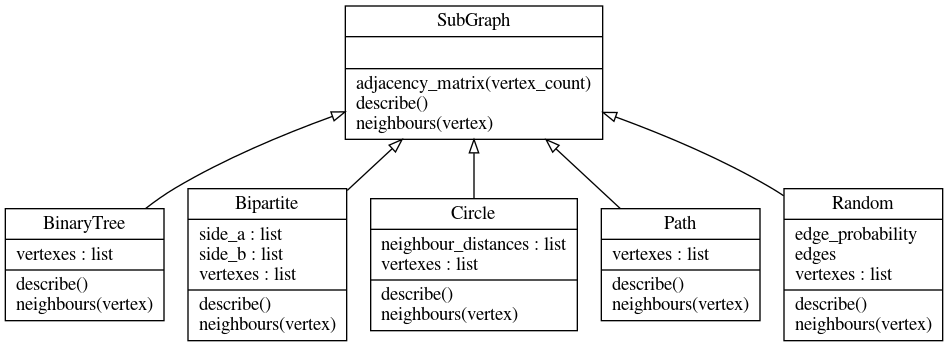
\includegraphics[width=\linewidth]{./figures/subgraph.png}
\end{center}

Ezen részgráfokból épülnek fel az alábbi kompozit gráfok:
\begin{itemize}
  \item Dumbbell
  \item GluedBinary
\end{itemize}

\begin{center}
  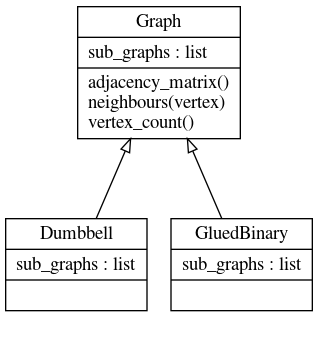
\includegraphics[width=0.4\linewidth]{./figures/graph.png}
\end{center}

\section{Szimulátorok}

A szimulátor osztályok közül a klasszikus tetszőleges kompozit gráfot tud
fogadni, a kvantumszimulátor jelenleg a kvantumbolyongás egy speciális
esetét, az egyenesen való bolyongást képes kezelni, mely a 2-regularitása miatt
egyszerűbben implementálható. Hosszú távú cél a k-reguláris, illetve az
általános gráfokra kiterjeszteni ezt a szimulátort.

\begin{center}
  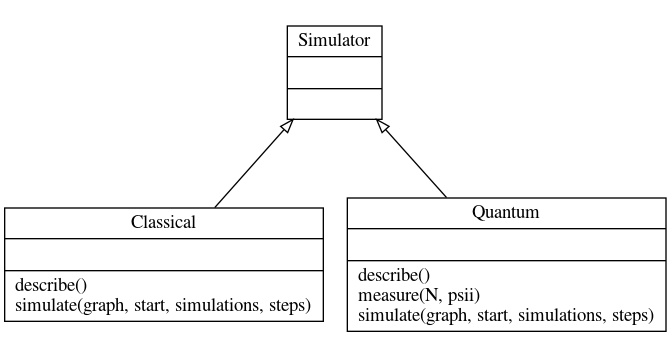
\includegraphics[width=0.8\linewidth]{./figures/simulator.png}
\end{center}

\section{Futtatás, konfiguráció, eredmények ábragenerátora}

A fenti osztályok segítségével egy olyan keretrendszert alakítottam ki, melyben
nagyon gyorsan fel lehet 1-1 futtatást konfigurálni. A futtatás eredményeit egy
összesített Latex dokumentumba gyűjti a program. Ez tartalmazza a beadott gráf
részgráfjainak nevesített típusát, szomszédossági mátrixait, illetve a teljes
gráf szomszédossági mátrixát, valamint a szimulációk eloszlási eredményeit. A
következő fejezetben több ilyen ábrát is bemutatok.

\chapter{Szimulációk, eredmények}

Ábrák értelmezése:

A lenti ábrákon a matplotlibes plazma színezésnek megfelelően a hidegebb (kék)
árnyalatok kisebb értéket, a melegebb (lila, majd sárga) árnyalatok magasabb
értékeket jelölnek. A fehér szín a 0 értéket jelöli.

A gráfok és részgráfok ábrái $n \times n$-es szomszédossági mátrixokat
ábrázolnak. A fehér cellák a nem-élek, a kék cellák az $1$-es súlyú élek.

A szimulációk ábráinak az $x$ tengelyén a gráfok csúcsai helyezkednek el
kiterítve, index szerinti növekvő sorrendben, az $y$ tengelyen a szimuláció
lépései helyezkednek el, alul a $0.$ lépés, felül az utolsó lépés.

\section{Súlyzó gráf}

Például egy súlyzó gráfról a következő képek készültek:

\begin{figure}[H]
  \centering
  \begin{subfigure}{.3\linewidth}
    \centering
    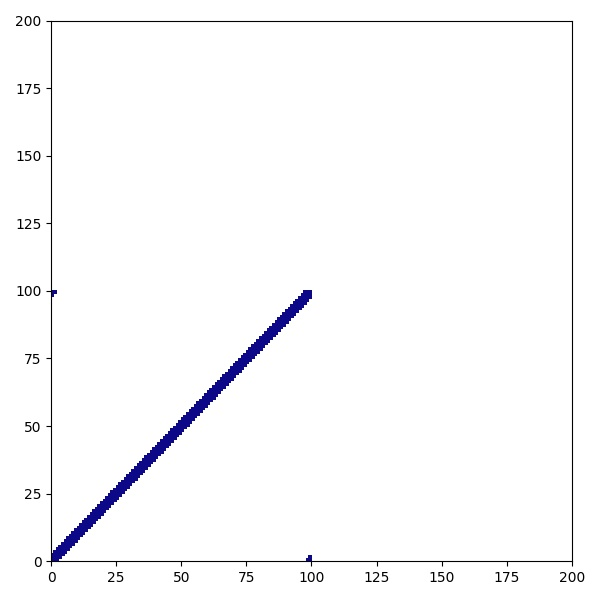
\includegraphics[width=\linewidth]{./figures/sulyzo/subgraph_00.jpg}
    \caption{Bal kör}
    \label{fig:sub1}
  \end{subfigure}
  \begin{subfigure}{.3\linewidth}
    \centering
    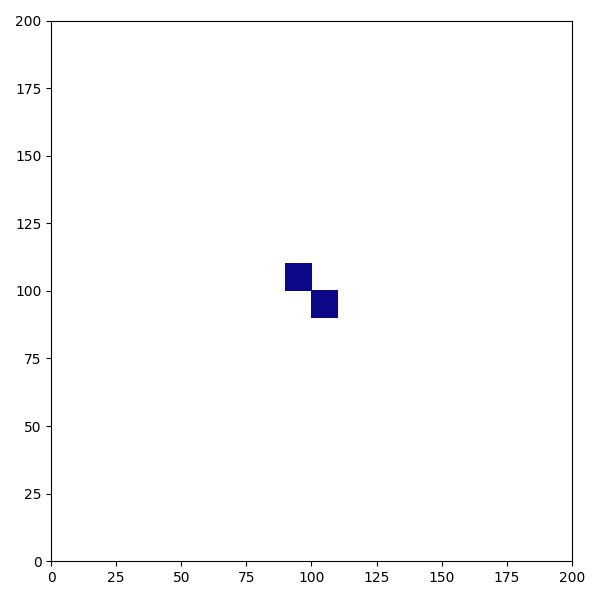
\includegraphics[width=\linewidth]{./figures/sulyzo/subgraph_02.jpg}
    \caption{Középső teljes páros gráf}
    \label{fig:sub2}
  \end{subfigure}
  \begin{subfigure}{.3\linewidth}
    \centering
    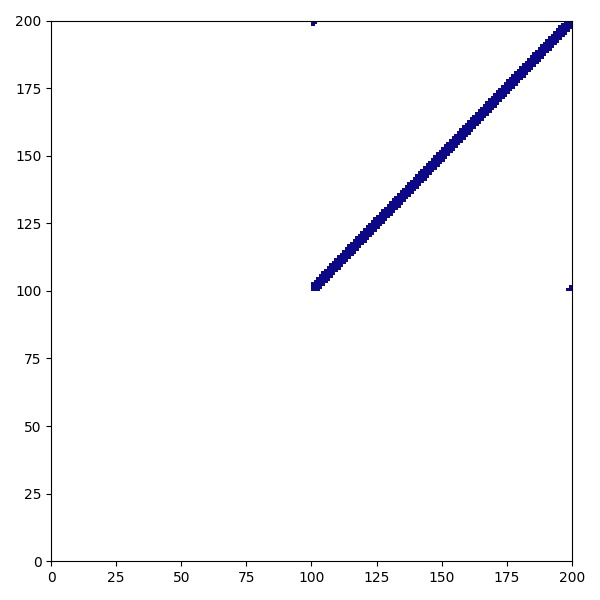
\includegraphics[width=\linewidth]{./figures/sulyzo/subgraph_01.jpg}
    \caption{Jobb kör}
    \label{fig:sub3}
  \end{subfigure}
  \caption{Súlyzó gráf részgráfjai}
  \label{fig:all}
\end{figure}

\begin{figure}[H]
  \centering
  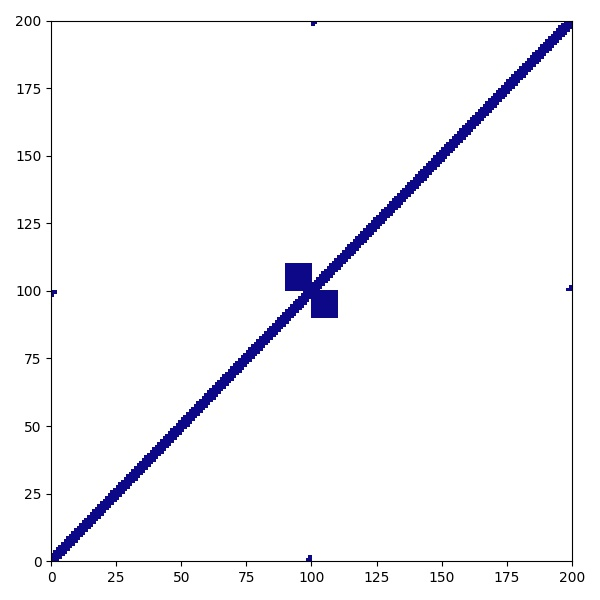
\includegraphics[width=0.5\linewidth]{./figures/sulyzo/graph.jpg}
  \caption{Súlyzó gráf}
\end{figure}

\begin{figure}[H]
  \centering
  \begin{subfigure}{.45\linewidth}
    \centering
    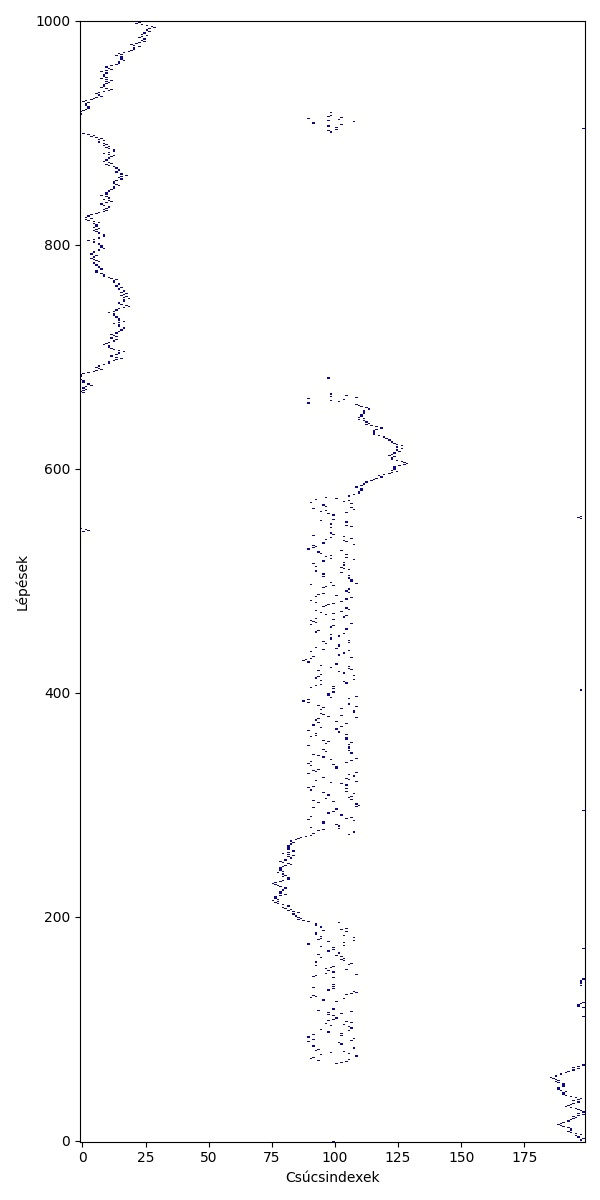
\includegraphics[width=\linewidth]{./figures/sulyzo/sim00.jpg}
    \caption{1 bolyongó}
  \end{subfigure}
  \begin{subfigure}{.45\linewidth}
    \centering
    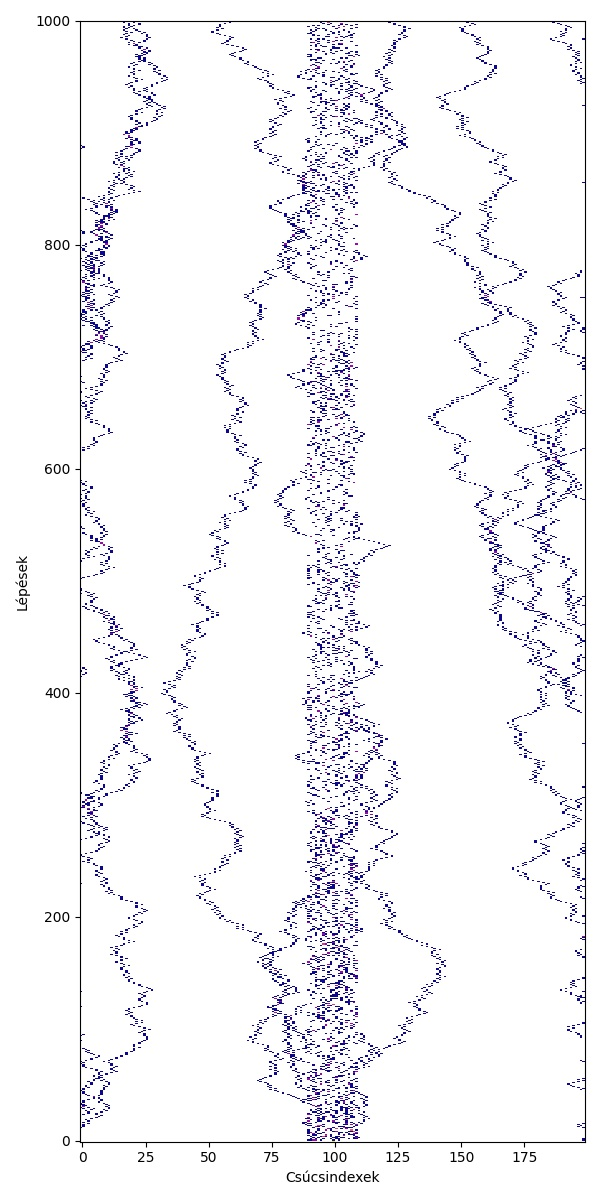
\includegraphics[width=\linewidth]{./figures/sulyzo/sim01.jpg}
    \caption{10 bolyongó}
  \end{subfigure}
\end{figure}

\begin{figure}[H]
  \centering
  \begin{subfigure}{.45\linewidth}
    \centering
    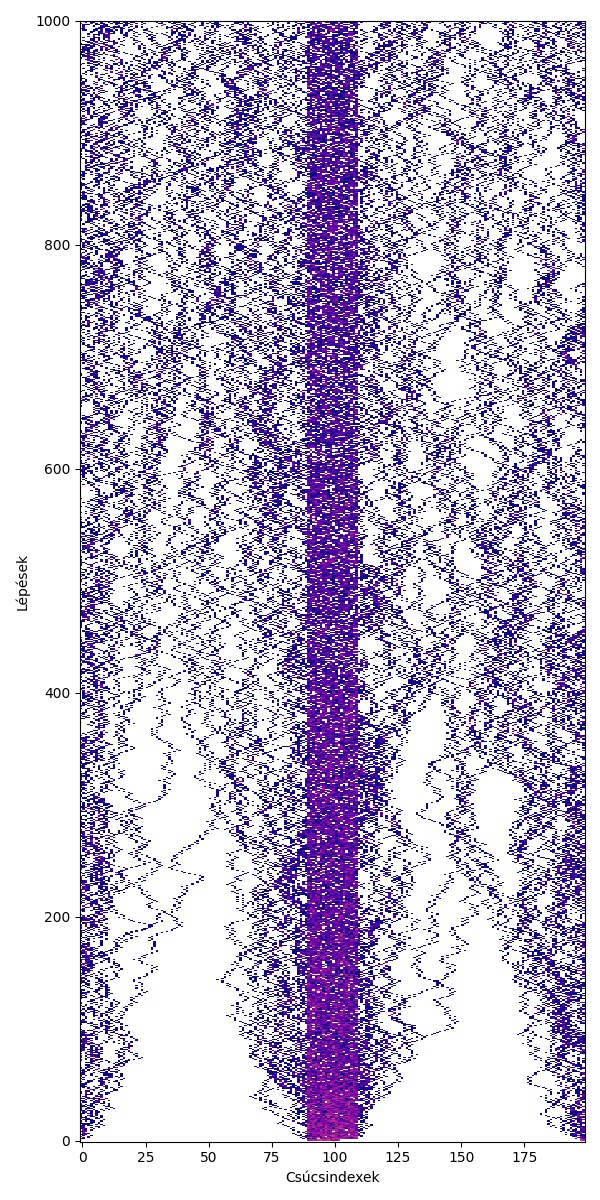
\includegraphics[width=\linewidth]{./figures/sulyzo/sim02.jpg}
    \caption{100 bolyongó}
  \end{subfigure}
  \begin{subfigure}{.45\linewidth}
    \centering
    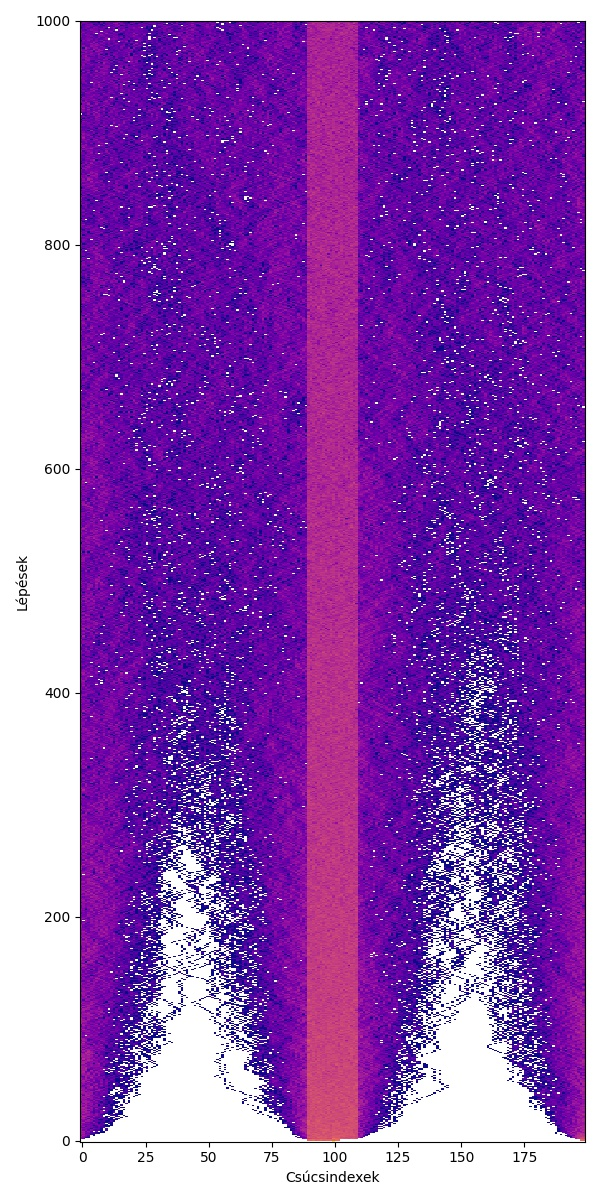
\includegraphics[width=\linewidth]{./figures/sulyzo/sim03.jpg}
    \caption{1000 bolyongó}
  \end{subfigure}
\end{figure}

\section{Ragasztott bináris fa}

\begin{figure}[H]
  \centering
  \begin{subfigure}{.3\linewidth}
    \centering
    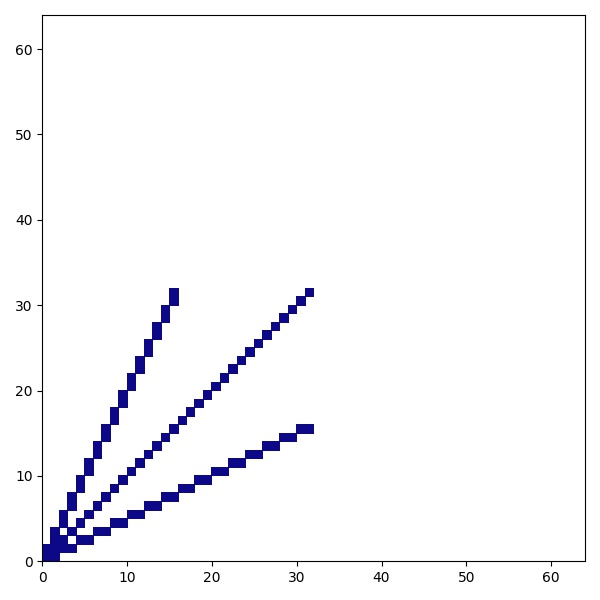
\includegraphics[width=\linewidth]{./figures/ragasztott_binaris/subgraph_00.jpg}
    \caption{Bal bináris fa}
  \end{subfigure}
  \begin{subfigure}{.3\linewidth}
    \centering
    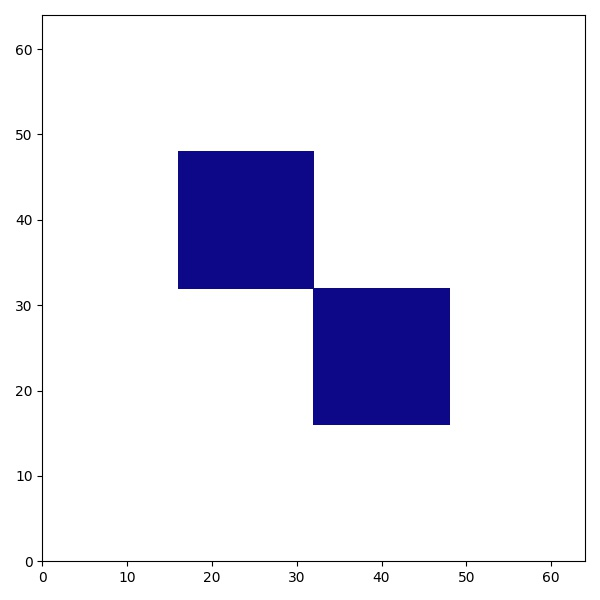
\includegraphics[width=\linewidth]{./figures/ragasztott_binaris/subgraph_02.jpg}
    \caption{Középső teljes páros gráf}
  \end{subfigure}
  \begin{subfigure}{.3\linewidth}
    \centering
    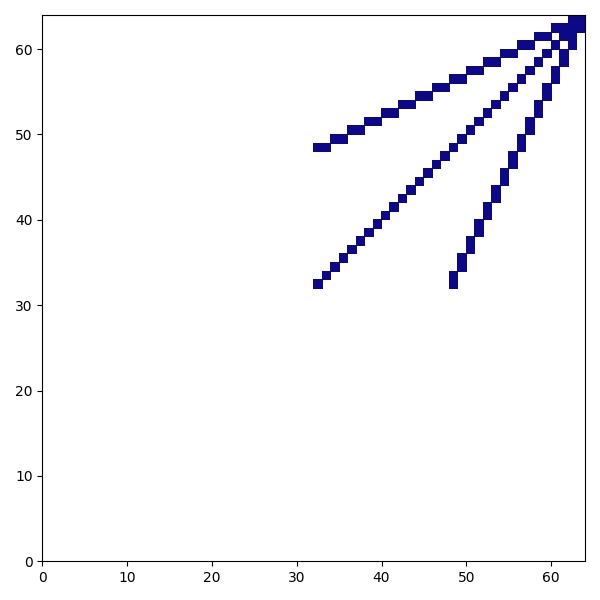
\includegraphics[width=\linewidth]{./figures/ragasztott_binaris/subgraph_01.jpg}
    \caption{Jobb bináris fa}
  \end{subfigure}
  \caption{Ragasztott bináris fa részgráfjai}
\end{figure}

\begin{figure}[H]
  \centering
  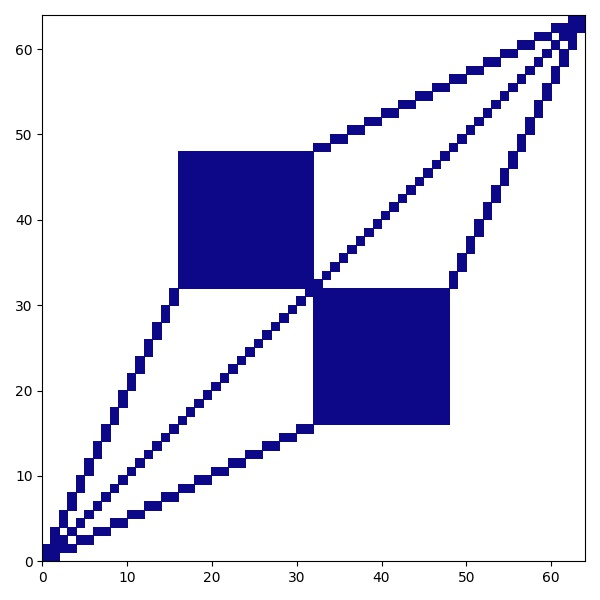
\includegraphics[width=0.5\linewidth]{./figures/ragasztott_binaris/graph.jpg}
  \caption{Ragasztott bináris fa}
\end{figure}

\begin{figure}[H]
  \centering
  \begin{subfigure}{.45\linewidth}
    \centering
    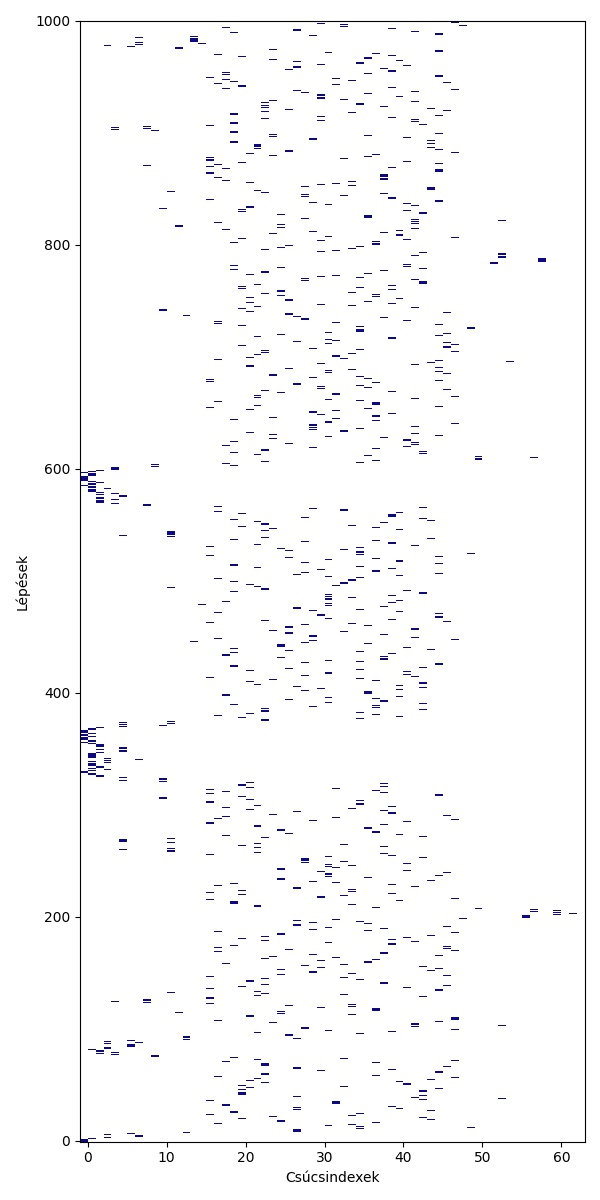
\includegraphics[width=\linewidth]{./figures/ragasztott_binaris/sim00.jpg}
    \caption{1 bolyongó}
  \end{subfigure}
  \begin{subfigure}{.45\linewidth}
    \centering
    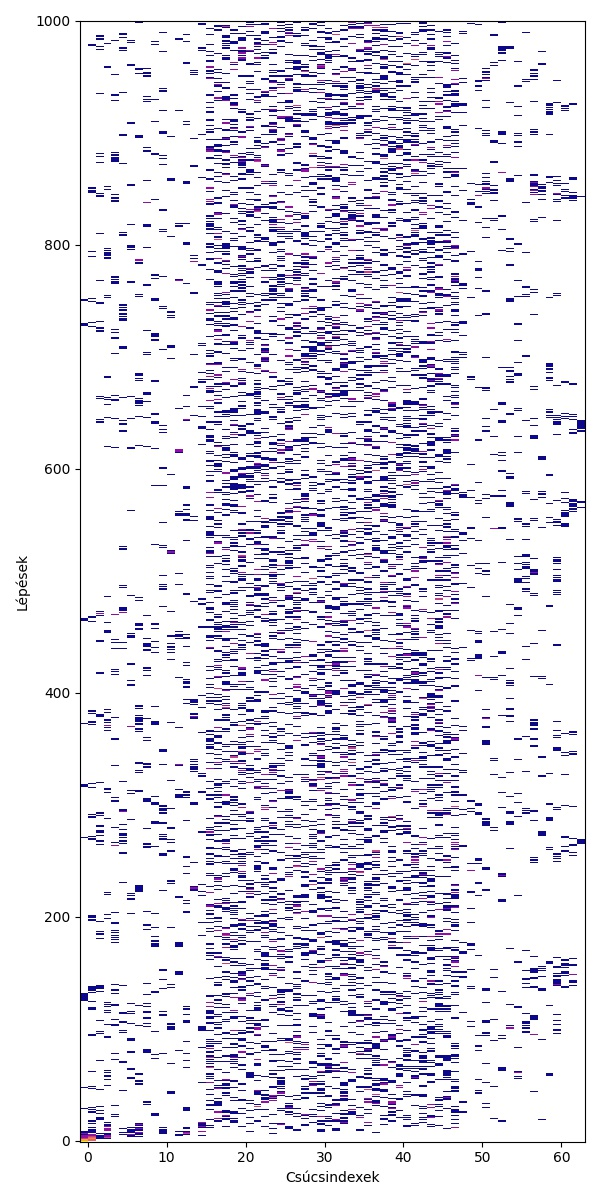
\includegraphics[width=\linewidth]{./figures/ragasztott_binaris/sim01.jpg}
    \caption{10 bolyongó}
  \end{subfigure}
\end{figure}

\begin{figure}[H]
  \centering
  \begin{subfigure}{.45\linewidth}
    \centering
    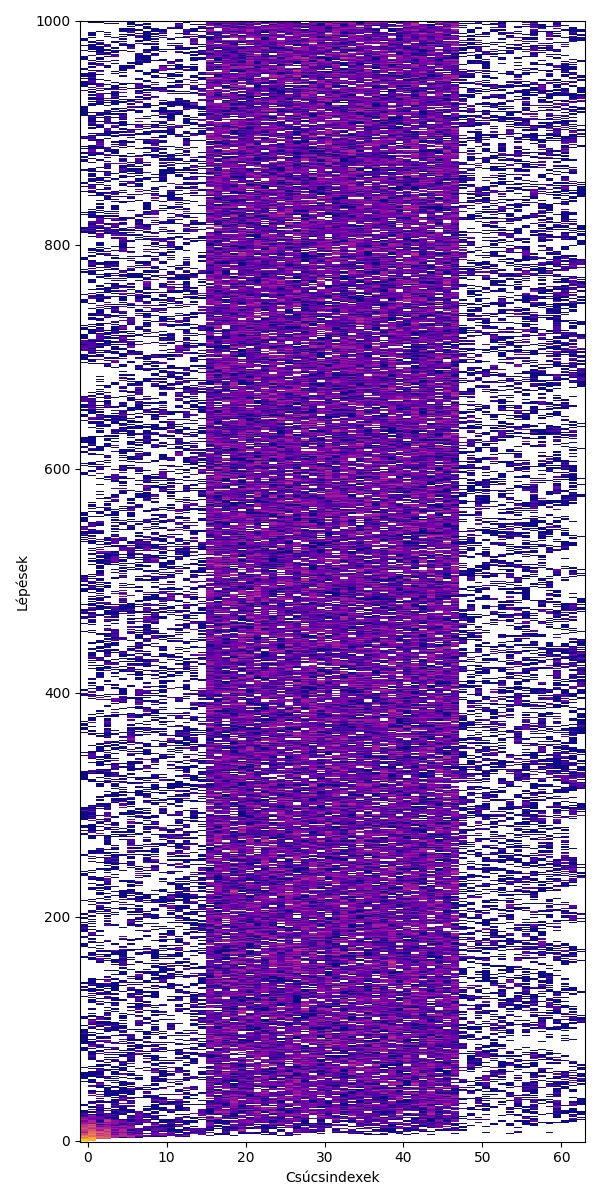
\includegraphics[width=\linewidth]{./figures/ragasztott_binaris/sim02.jpg}
    \caption{100 bolyongó}
  \end{subfigure}
  \begin{subfigure}{.45\linewidth}
    \centering
    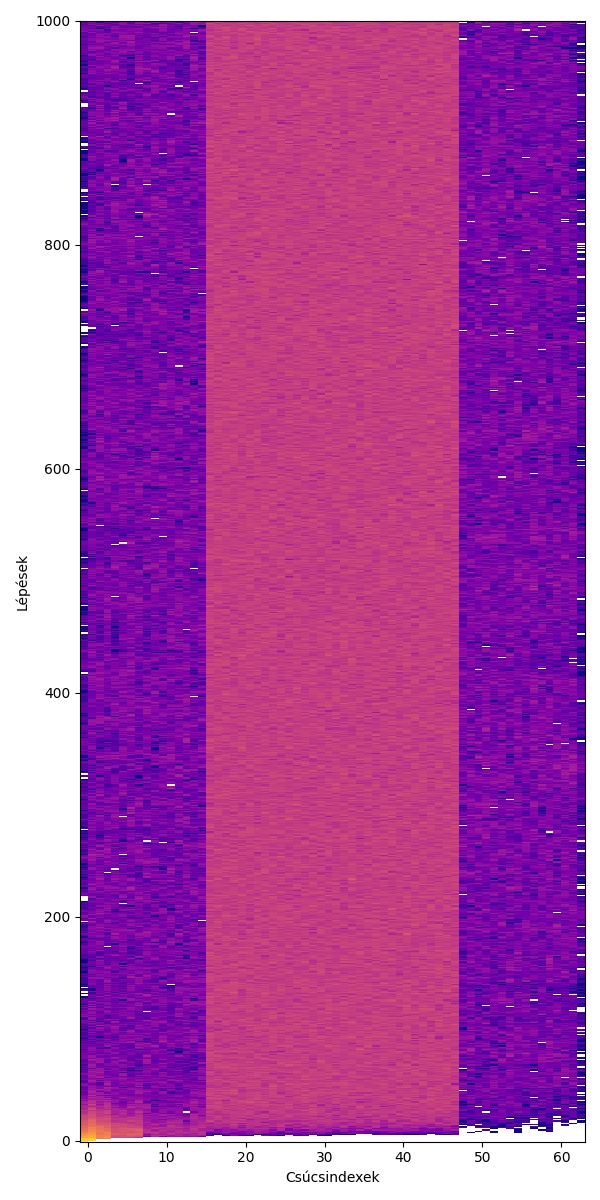
\includegraphics[width=\linewidth]{./figures/ragasztott_binaris/sim03.jpg}
    \caption{1000 bolyongó}
  \end{subfigure}
\end{figure}

\section{Bolyongás az egyenesen, klasszikus és kvantum esetben}

\begin{figure}[H]
  \centering
  \begin{subfigure}{.45\linewidth}
    \centering
    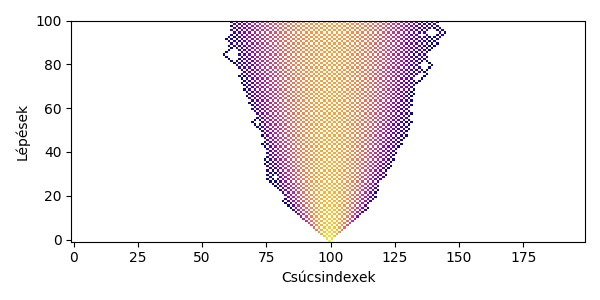
\includegraphics[width=\linewidth]{./figures/quantum/classical_simulation_short.jpg}
    \caption{Klasszikus}
  \end{subfigure}
  \begin{subfigure}{.45\linewidth}
    \centering
    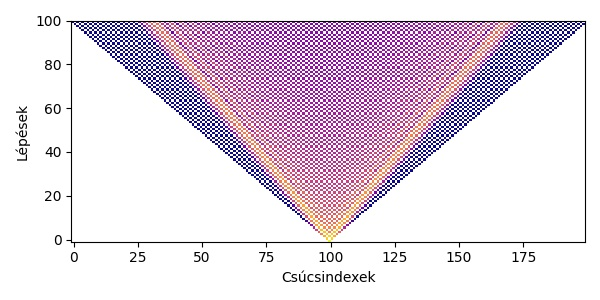
\includegraphics[width=\linewidth]{./figures/quantum/quantum_simulation_short.jpg}
    \caption{Kvantum}
  \end{subfigure}
\end{figure}

Kijött a szokásos klasszikus és kvantum közötti különbség, a klasszikus az
origó körül csúcsosodik, a kvantum viszont "2 púpú teve" szerű eloszlást mutat.

\begin{figure}[H]
  \centering
  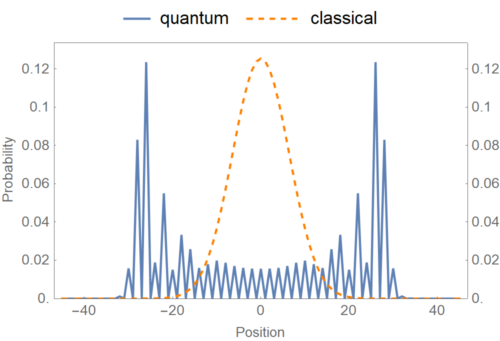
\includegraphics[width=0.5\linewidth]{./figures/quantum/teve.png}
  \caption{Eloszlások különbözősége \cite{VicPina}}
\end{figure}

\section{Bolyongás a szakaszon, klasszikus és kvantum esetben}

A szakasz végpontjai visszatükrözik a bolyongót.

\begin{figure}[H]
  \centering
  \begin{subfigure}{.45\linewidth}
    \centering
    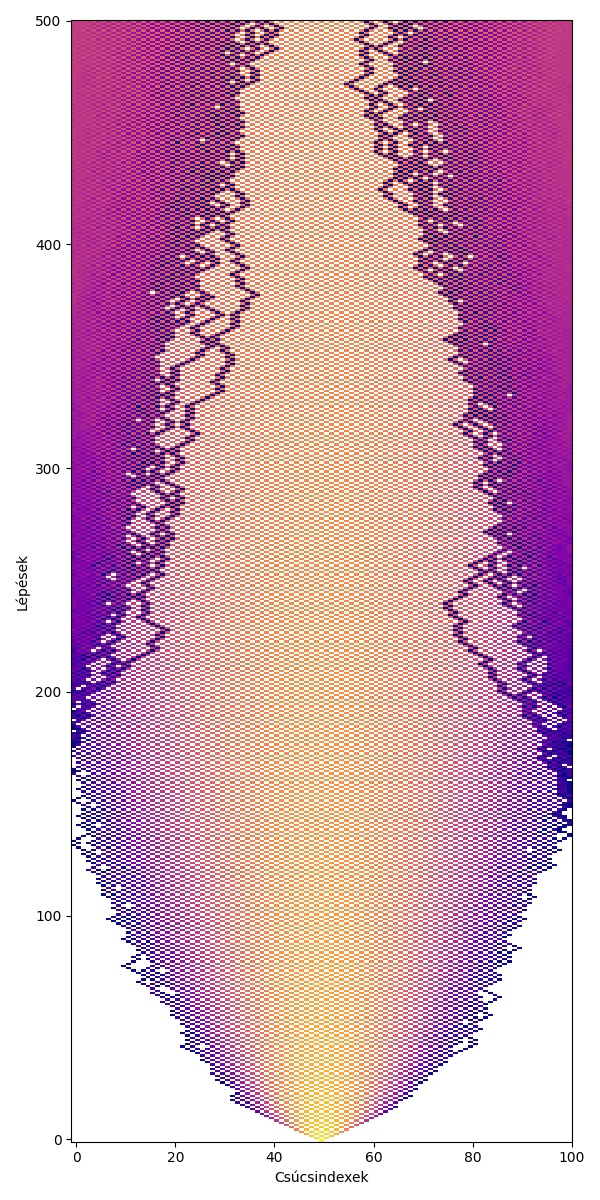
\includegraphics[width=\linewidth]{./figures/quantum/classical_simulation_long.jpg}
    \caption{Klasszikus}
  \end{subfigure}
  \begin{subfigure}{.45\linewidth}
    \centering
    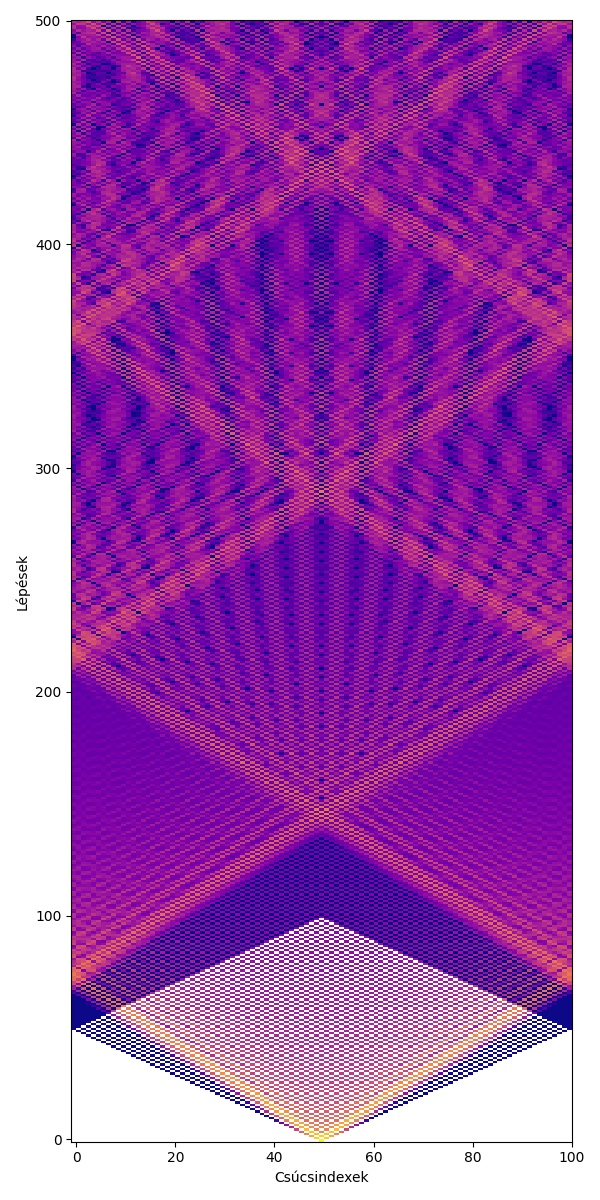
\includegraphics[width=\linewidth]{./figures/quantum/quantum_simulation_long.jpg}
    \caption{Kvantum}
  \end{subfigure}
\end{figure}
\chapter{Jövőbeli tervek}

\begin{itemize}
  \item Elolvasni a Springer sorozatos kvantumbolyongós könyveket.
  \item Implementálni k-reguláris gráfra a bolyongást.
  \item Implementálni általános gráfra a bolyongást.
  \item Számolni hitting time-ot és mixing rate-t.
  \item Számolni a szomszédossági mátrixból sajátértékeket és azokat elemezni.
  \item Számolni határeloszlást a Markov-láncokhoz.
  \item Súlyozott éleket használni (hurokéllel).
\end{itemize}

\nocite{*}

Források (rendesen hivatkozva majd...):
\begin{itemize}
  \item Hirvensalo könyv
  \item http://susan-stepney.blogspot.com/2014/02/mathjax.html (Ezt nyáron lecserélni rendes cikkre.)
\end{itemize}

\addcontentsline{toc}{chapter}{\bibname}
\bibliography{bib/mybib}

\end{document}